% Created 2022-02-08 Tue 12:50
% Intended LaTeX compiler: pdflatex
\documentclass[11pt]{article}
\usepackage[utf8]{inputenc}
\usepackage[T1]{fontenc}
\usepackage{graphicx}
\usepackage{longtable}
\usepackage{wrapfig}
\usepackage{rotating}
\usepackage[normalem]{ulem}
\usepackage{amsmath}
\usepackage{amssymb}
\usepackage{capt-of}
\usepackage{hyperref}
\author{Thorvald Ballestad}
\date{\today}
\title{WIP Notes on Weyl and Dirac semimetals}
\hypersetup{
 pdfauthor={Thorvald Ballestad},
 pdftitle={WIP Notes on Weyl and Dirac semimetals},
 pdfkeywords={},
 pdfsubject={},
 pdfcreator={Emacs 27.2 (Org mode 9.6)}, 
 pdflang={English}}
\begin{document}

\maketitle
\tableofcontents

See meeting \href{file:///home/thorvald/Documents/NTNU/10semester/meetings/01-17.org}{Type II SM} for initial notes about this


\section{Outline of section -- Type II}
\label{sec:orgcffdb16}
This is partially based on the notes written on the meeting \href{file:///home/thorvald/Documents/NTNU/10semester/meetings/01-17.org}{01-17}

\subsection{History}
\label{sec:org070ad8a}
soluyanovTypeIIWeylSemimetals2015 first described these.
The possibility of tilting the cone below the plane, giving conic sections with finite length, had not been considered before.
In high energy phsycics this makes no sense, as it would break lorentz invairance (describe in more depth. See \hyperref[sec:orgde4474d]{Breaking Lorentz invariance}).
In condensed matter physics, however, this is not an issue, and this tilting gives rise to a new class of weyl SM.
The transition from type i to type ii is a critical/phase/abrupt transition, as the fermi surface goes from a point to a finite line.
This gives rise to different material properties (cite, cite, cite), as the density of states is finite (check) due to the electron and hole pockets now being at the fermi level (define what these pockets are).

Maybe mention some of the original predictions made about type ii, and whether or not they were correct.

Can take inspiration from \hyperref[sec:org7941e69]{Weyl SM YT video}  \emph{Note: the talk is actually about Weyl semimetals in general, not only type ii}

\begin{quote}
The problem of the conic section of a plane restricted to pass through the node of the cone is trivially seen to have two solutions: a point and two intersecting lines.
Despite this, the possibility of a Weyl cone tilted such that the bands crosses the Fermi surface was never considered before Soluyanov et al described this new class of Weyl semimetals in 2015.
This now seemingly obvious possibility made an already rich field even more exciting, opening up for a wider range of novel and interesting effects (some examples or cites).
\end{quote}

\subsection{Hamiltonian}
\label{sec:org547238c}
Firstly show example of realistic Hamiltonian of a Weyl SM, with a tunable parameter going from type I to type II.
See also \hyperref[sec:org855f368]{Inclusion of more realistic energy dispersion for a Weyl SM} and the ridgeline plot in \hyperref[sec:orgc5c2be2]{Ridgeline plot}
Around each of the nodes, the Hamiltonian may be linearized, giving the simple model of the linearized dirac cone, which perfectly matches its high energy equivalent particle -- the massless fermion.
These linearized models are much easier to work with, and does well in describing the low energy interaction/behavior of the system.

\subsection{Eigenvalues and -states}
\label{sec:org22909e4}
Find the eigenvalues.
Find spin states
See \hyperref[sec:org6b31ee0]{Eigenvalues and eigenstates}
Berry curvature
See also \hyperref[sec:org855f368]{Inclusion of more realistic energy dispersion for a Weyl SM} 

\subsubsection{Landau level description}
\label{sec:org00cdc6a}
Landau level description only valid for certain directions of the B field for a type II sm
Outside of the region of validity the levels break down, and some other basis must be used.
Worth to mention that this confused the original discoverers of the Tyep II to believe the chiral anomaly did not hold for certain directions, but later calculations has proved otherwise.

Can use the very pretty figures showing the regions of validity of the LL
\begin{center}
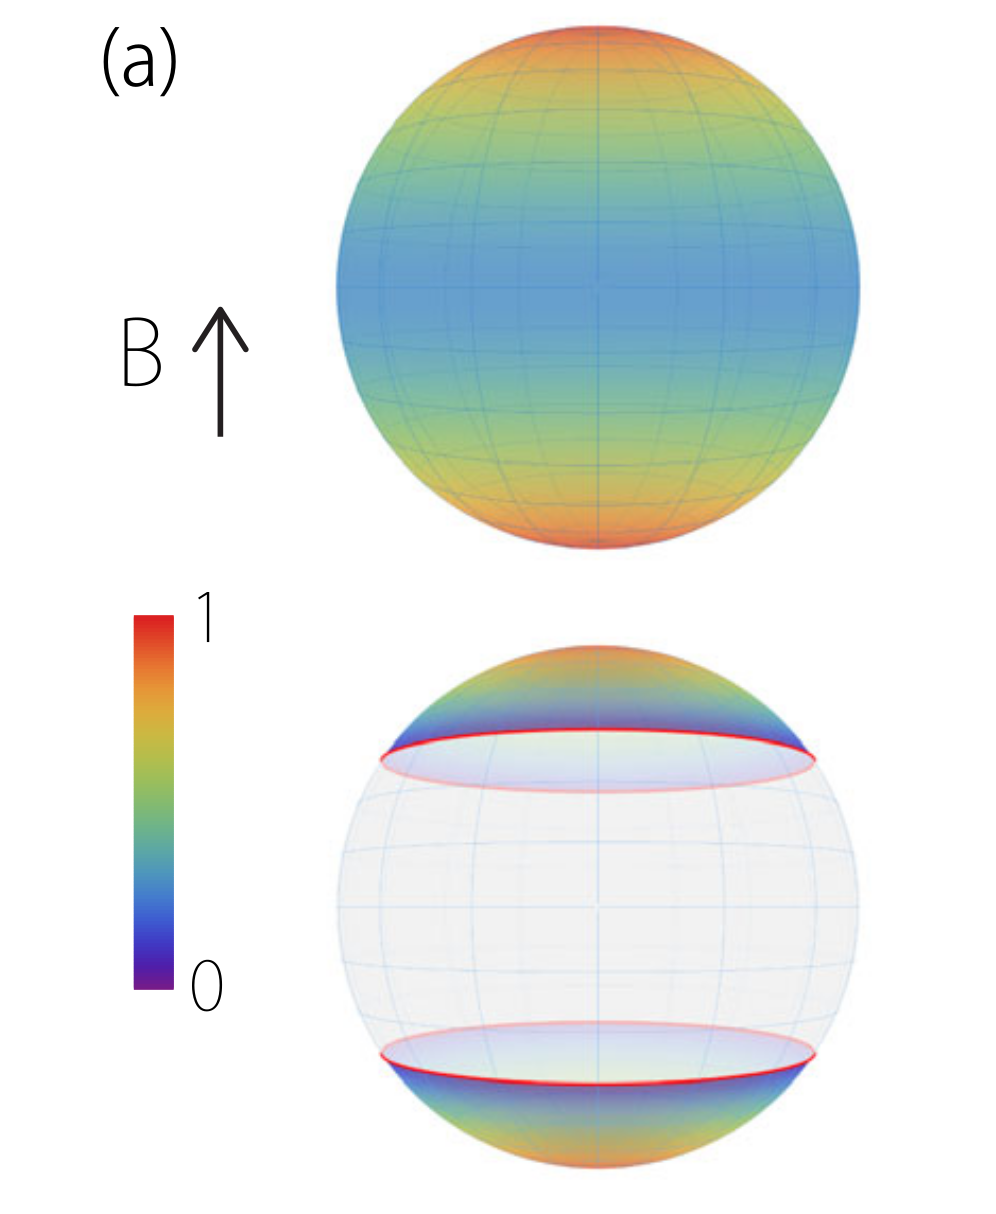
\includegraphics[width=.9\linewidth]{figures/typeii_ll_region_yu.png}
\end{center}

\begin{center}
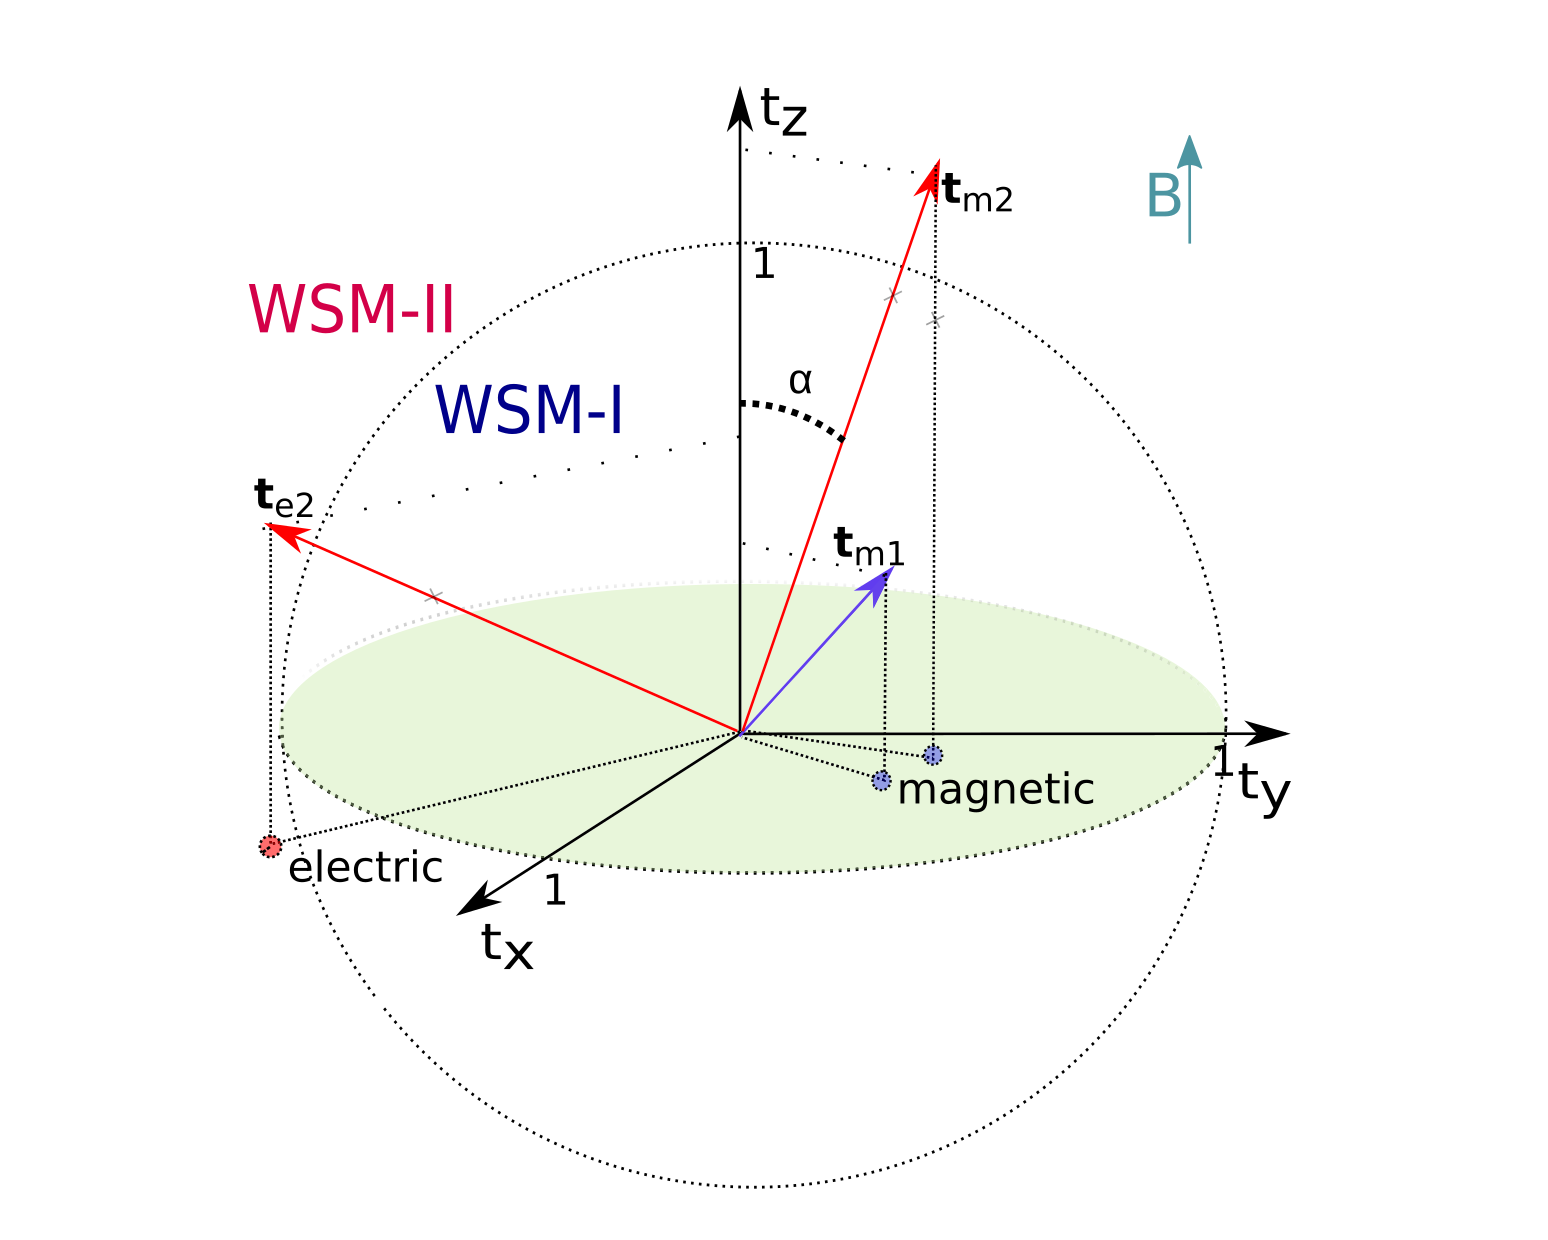
\includegraphics[width=.9\linewidth]{figures/typeii_ll_region_Tchoumakov.png}
\end{center}

In the project thesis we did fin the LL of a untilted system, with quite a manual approach
Apparently, this is not the best solution, and Tchoumakov et al for example write \emph{while the Hamiltopnian can, in principle, within a lengthy calculation, be solvbed by the introduction of the ladder operators, \ldots{}. a more elegant methjod consist of usign t a hyperbocli trransofrmation to change teh eigenvalue eqaution}
Probaby better to use that formulation

\begin{enumerate}
\item {\bfseries\sffamily TODO} Find the LL of untilted WP using the boost
\label{sec:orgf8c406f}
It might be that this does not make sense, and that the purpose of the boost is simply to get it into a frame where we have an untilted cone.
\emph{Yes, I think this is the case}

\item {\bfseries\sffamily TODO} Fidn the LL of tilted WP using the boost
\label{sec:orgcf34e8e}
The issue to be solved is that for the tilted system we have qx/qy present in the diagonal of our hamiltonian, and wer are thus unable to use the ladder operator approach.
However, we may use a boost to transform our Hamiltonian to a form where qx/qy are restricted to the off-diagonal elements.
\end{enumerate}

\subsubsection{Plot}
\label{sec:org94d1b5e}

\subsubsection{Fermi Arc?}
\label{sec:org9c982e6}

\subsection{Show calculation of Chiral anomaly?}
\label{sec:org25ef014}
Done using quasiclassical theory.
Original paper's issue when using LL

\subsection{Interpretation of the states dipping through the plane (pockets)}
\label{sec:orgf8fbf90}

\subsection{Material realizations}
\label{sec:org332ac94}


\section{Eigenvalues and eigenstates}
\label{sec:org6b31ee0}

\subsection{{\bfseries\sffamily DONE} Show the eigenstates as well as values for a Dirac SM.}
\label{sec:orgc3402d6}
Should show how the spin behaves on the cone, probably similar to a Rashba.
This is useful showing more explicilty the chirality of the cones?

\subsubsection{{\bfseries\sffamily DONE} Without v\textsubscript{f}}
\label{sec:orgcce7273}
We did this, and found the spin expectation values to be \((k_x, k_y, k_z)\).
See \url{file:///home/thorvald/Documents/NTNU/10semester/mathematica/Spin\_state\_weyl.nb} and notes on Remarkable

\subsubsection{{\bfseries\sffamily DONE} With v\textsubscript{f}}
\label{sec:org9f6edc7}

\subsection{Notes about the eigenstates}
\label{sec:org1e85d39}
The expectation value of the spin we arrived at takes the shape of a ``hedgehog'', or a source/sink.
This corresponds exactly with the theory of Berry curvature/charge, and the topological nature of the Weyl points.
Is this coincidental or is there a relation/even the exact same thing?
See more in burkovTopologicalSemimetals2016b.

The expectation value of the spin in a rashba system, as shown in the project thesis, takes the form of a rotating field around the origin.
Can we relate this to berry curvature or some topological quantity as well?
d

\subsection{Ridgeline plot}
\label{sec:orgc5c2be2}
Using the Hamiltonian in sharmaChiralAnomalyLongitudinal2017 we found the eigenvalues of a more realistic model of a Type II weyl sm and plotted the transition from at type I to a type II.
See \href{file:///home/thorvald/Documents/NTNU/10semester/mathematica/TYPEII\_model.nb}{Notebook on the TypeII model}, and the figure \href{figures/typeIIridgeline.png}{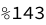
\includegraphics[width=.9\linewidth]{/home/thorvald/Documents/NTNU/10semester/notes/figures/typeIIridgeline.png}}


\section{Weyl SM YT video}
\label{sec:org7941e69}
\href{https://youtube.com/watch?v=Du5z7NEYYDw}{Talk about Weyl SM}
Nice intro we might use for an introduction or something, with nice words like discovery of the year and such

\subsection{Quick live notes}
\label{sec:orga34b071}
\begin{itemize}
\item The \emph{fermion trio} completed with Dirac(2005), Majonara(2012), and Weyl(2015).
Maybe interesting to briefly note what Majonara Fermions are?
\item Some confusion to 2D vs 3D. Seems like he calls 2D (graphene) Dirac and 3D Weyl.
Am I mistaken, does he use out of date terminmology or is there several contradictory terminmologies out there?
\item What are right and left movers in 3D?
This is related to the chirality of the weyl points. What is the chirality in three (or event two) dim? \label{dim_discussion}
\item Surface state gives spiral motion in real space
Why? I don't understand this
\item Realistic Hamiltonian.
In the project thesis we used the simplest expansion of a cone around the weyl point.
Would it be interesting to use a more realistic Hamiltonian, valid for a larger region of the Brillouine zone?
\item Landauer formula vs. Kubor formula
Could this be a better way to do stuff?
\end{itemize}


\section{Type II - Quick notes}
\label{sec:org58a78a6}
First described in soluyanovTypeIIWeylSemimetals2015, quite well written.
Can write about classification, thermodynamic properties, the fact that the chiral anomaly is broken if the magnetic field is not in a certain direction.

Should better understand what hole and electron pockets are

\subsection{Classification Type I and Type II}
\label{sec:orgbcd00f2}
Refer to quadric surfaces and conic sections.
See for example \url{https://link.springer.com/content/pdf/10.1007\%2F978-1-4612-4390-8.pdf} p. 195

\subsubsection{In two dimensions}
\label{sec:org8388d37}
In two dimensions this is the conic intersection problem.
Specifically, as the plane of intersection passes through the origin, we have the degenerate conic intersection.
It is a matter of definition if this case is included in the conic intersections, so this is important to be aware of.
However, the solutions to the degenerate conic intersection is simple, and we straight out get a set of cases.
We may use these to show that is must be one of two cases.

\subsubsection{In three dimension}
\label{sec:orgcaec31d}
I believe it is here also the \emph{degerate} quadric surface problem, but I don't really know.
Probably important to check that the degerate case is included in whatever formalism one uses for categroization.
Anyways, the link above should probably give some good insight.

\subsection{What is the interpretation of the states ``dipping'' through the plane?}
\label{sec:org29cec00}
We reffer to these as electron and hole pockets, I believe, but what is the interpretation of this and which physical consequences does it have?

\subsection{Breaking Lorentz invariance}
\label{sec:orgde4474d}
Explicitly show how the lorentz invairance is broken
All sources state that the lorentz invariance is broken when over-tilting a cone, but would be nice to show explicilty
Also somewhere noted that when the velocity is the fermi velocity and not the speed of light, lorentz invairance is broken anyways

\subsection{Anoamly and Landau levels}
\label{sec:orgada1378}

\sout{The chiral anomaly is not preserved in Type II if the magentic field is of a certain direction.
This has to do with the landau levels being gapped, so it is probably an issue for us as well.}
The results foun by Burkov that the chiral anomaly does not hold for certain directions of the magnetic field was mistaken.
As was shown by sharmaChiralAnomalyLongitudinal2017, the calculation done by Burkov was too naive.

\subsection{Fermi arc}
\label{sec:org850f04a}
What is a Fermi arc?
\begin{itemize}
\item Talked about in YouTube video \hyperref[sec:org7941e69]{Weyl SM YT video}, where he discusses Fermi circle vs arc.
\item Generally called Fermi contours
\end{itemize}

\subsection{Source of the tilting vector}
\label{sec:orgb0a8226}
What is the physical origin of the tilt/tilting vector?
It is to some degree material spesific, but is it also dependent on for example externally applied fields

\subsection{Conic seciton not at the ``origin''}
\label{sec:org0714e07}
If the Fermi level is above (below) the dirac node, will not the conic seciton be more exotic?

\section{Collapse of Landau levels in Weyl semimetals}
\label{sec:org98006f5}
\subsection{Collapse of LL and pseudo LL}
\label{sec:org9f33a90}
arjonaCollapseLandauLevels2017
What on earth are pseudo LL (landau levels)?

\section{Conformal anomaly in Type II weyl SM}
\label{sec:org782ec04}

\subsection{Thoughts}
\label{sec:orgfee921d}

\subsubsection{Inclusion of more realistic energy dispersion for a Weyl SM}
\label{sec:org855f368}
I think a better structure of the section on weyl sm i sto first present a more realistic dispersion relation, and then show how we may linaearize the cones about the node points.
This also illustrates clearly how the cones should be tilted in realtion to each other etc.

\subsection{Landau levels}
\label{sec:org978a228}
The issue with Type II Weyl SM is that the Landau level description collapses for certain directions of the magnetic field.
For type I all directions are compatible with LL, but for Type II only some directions are.
This caused for example the original paper describing Type II to mistakenly believe that the Chiral anomaly would only be present for certian directions of the B field, however, as was shown later, this was an errenous conclusion caused by not recognizing the collapse of the LL.
A quasiclassical computation showed that the Chiral anomaly is present for all directions of the magnetic field, and that one observes no critical effects at the transition between Type I and Type II.
As far as I understood, the quasiclassical approach was able to include the effects of the anomaly by including an axion term, the origin of the chiral anomaly.
If we were to try something similar, we would, I think, have to find a similar term causing the conformal anomaly.
Whether such a term exists, I don't know.
We will, probably, be able to use the LL approach within the region of validity for the LL description.

\section{Nature Burkov}
\label{sec:org8028f8b}
burkovTopologicalSemimetals2016b
\subsection{Chiral anomaly}
\label{sec:orgcceb123}
Always see the chiral anomaly described in one dimesnion.
What are the states and what is the meaning of right and left movers when we are in two or three dimensions?
See also \ref{dim_discussion} above.

\textbf{Answer:}
The Landau levels are degenerate in \(k_x, k_y\) (for a B-field in the z-direction).
Thus, the Landau level energy spectrum is effectively one-dimensional, making the usual discussion perfectly sound.
\subsection{Supplementary material, anomaly dependence on direction}
\label{sec:orgf6ae5dd}

\subsubsection{Contradictory results?}
\label{sec:org159d6ba}
sharmaChiralAnomalyLongitudinal2017 writes
\texttt{It has been suggested that ... [the] chiral-anomaly-induced negative LMR is strongly anisotropic, vanishing when the applied magnetic field is perpendicular to the direction of tilt of Weyl fermion cones in a type-II WSM}
however
\texttt{We analyze chiral anomaly in a type-II WSM in a quasiclassical Boltzmann framework, and find that the chiral-anomaly-induced positive longitudinal magnetoconductivity is present along any arbitrary direction.}
Is this to be understood as them getting a contradictory result?
In that casek, we must find out who are right.

\textbf{It seems like the results found in Burkov was wrong}

\subsubsection{Figure 3}
\label{sec:orgef28dc9}
Is this figure wrong?
How did they get separation of the upper and lower energy levels?
\end{document}
